\chapter{PaaS Management}\label{paas-management}

This chapter describes the stack around a container-based production
environment, and how applications could take advantage on it.

\begin{figure}[htbp]
\centering
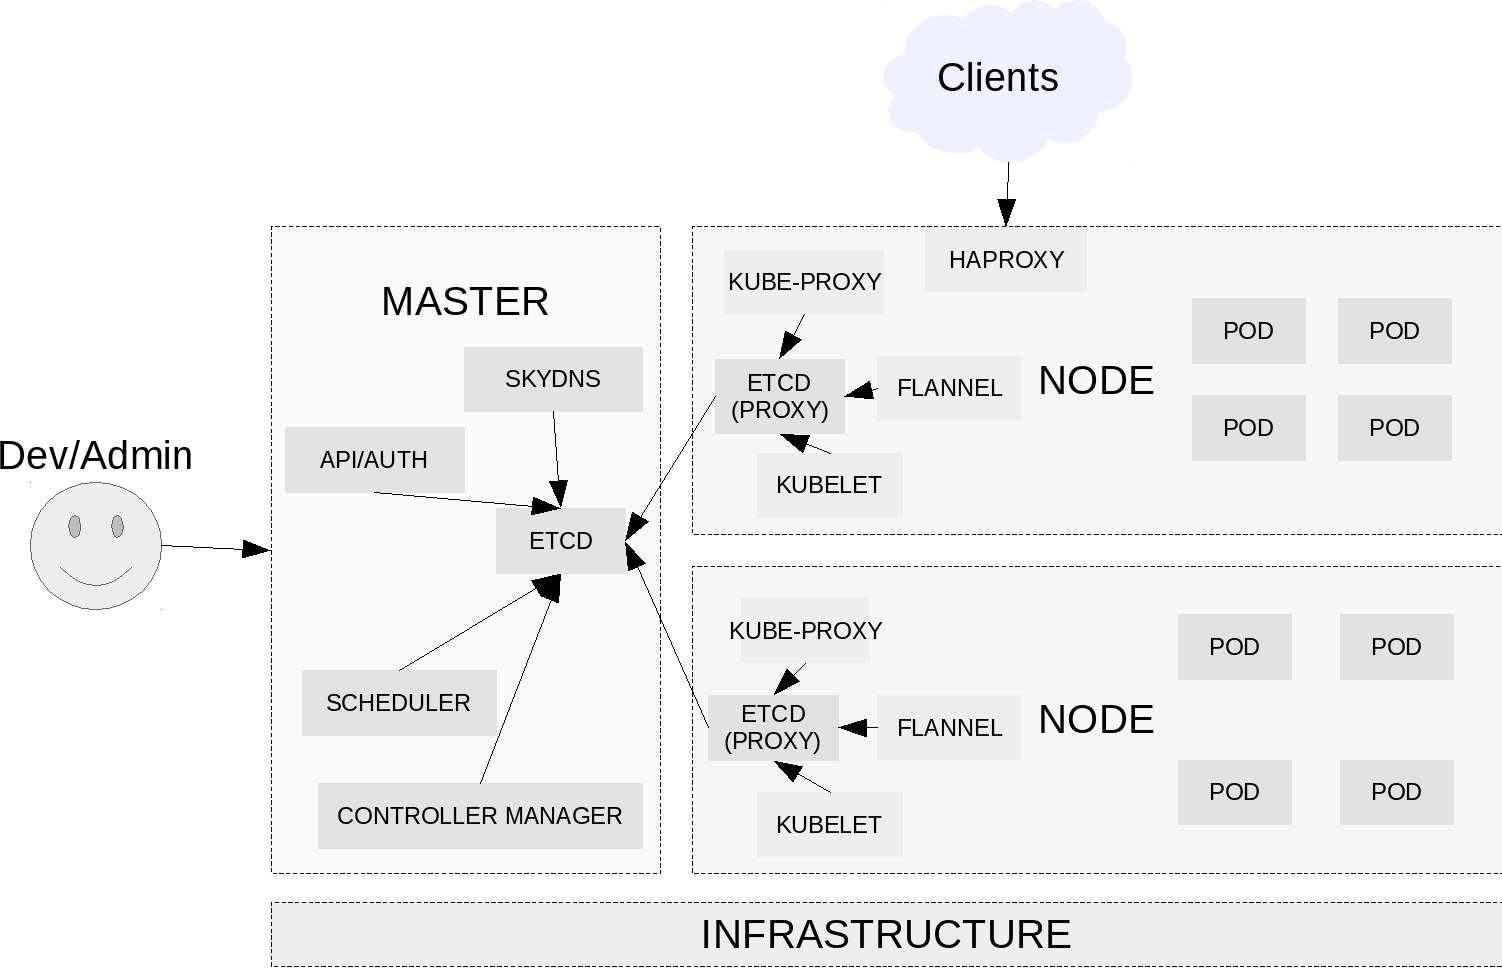
\includegraphics{media/ch5-overview.png}
\caption{Cluster Overview}
\end{figure}

\section{The Container Cluster's Core}\label{the-container-clusters-core}

In the container world, the operating system role should only be concerned in providing a minimal base for running containers.  In fact, since all the application dependencies are demanded to containers, there is only need of basic functionality, without a package manager and other features of a traditional OS.

The first and currently the most popular project that take into that direction has been \textit{CoreOS}, announced in summer 2013 as a Gentoo-based GNU/Linux distribution for deploying containers in a clustered environment. CoreOS occupies few memory and comes with \textit{SystemD}, \textit{Docker} and additional tools for distributed cluster environments like \textit{Etcd}.

\textit{SystemD} is the de-facto standard in GNU/Linux distribution as init daemon. SystemD made really easy to demonize processes and has advanced features such as parallelization and socket activation.  For example, the SSH daemon is stopped by default in order to save memory, and it will be started only after an incoming request on 22 TCP socket.  SystemD is used for running directly the OpenShift/Kubernetes binaries, outside containers, and the other core tools.

\textit{Etcd} is a key-value store which represent the database of the cluster since it has been used for inter-host communication by all components.  It could be used as a single master as in this project, or in high availability and distributed mode, useful for multi-master cluster configuration.

\textit{Fleet} provides a distributed init system, extending SystemD functionality from host-level to cluster-level.  Fleet has not been used in this case, but represent an alternative to Cloud Config in settings up the SystemD units.  In fact, it permits to bootstrap the OpenShift/Kubernetes stack from the master to all nodes.

\textit{Flannel} has been development as a requisites of the Kubernetes networking model, providing a subnet mask to every host in order to enable an overlay network for container inter-host communication.  At boot time, Flannet set the network data into Etcd under \texttt{/coreos.io} key.

CoreOS releases are organized in 3 channels: alpha, beta and stable. Alpha is generally release once a week and includes new software, while stable it's more suitable for production.

Most popular alternatives to CoreOS are Rancher OS (http://rancher.com/rancher-os/), Atomic (http://www.projectatomic.io/) by Red Hat and Ubuntu Snappy (http://www.ubuntu.com/cloud/tools/snappy) by Canonical.

\section{Microservices Scaling and Orchestration}\label{microservices-scaling-and-orchestration}

Kubernetes (http://kubernetes.io/) has been announced at Google I/O in June 2014, it's a cluster management system, a framework for container scheduling and orchestration in a clustered environment. Kubernetes has been developed by the same engineers who developed the current Google infrastructure, and takes advantage of that experience.  While CoreOS provides the basic for running containers, Kubernetes enables an higher level through the container scheduling and orchestration across all the cluster.

From the experience at Google, Kubernetes introduces some additional concepts on top of containers:
\begin{itemize}
\item \textit{pod}, a set of one or more containers that run together on a node, represents a single logic unit
\item \textit{replicationController} is concerned about guarantee the correct numbers of replicas of a pod
\item \textit{service} groups pods and provides a common DNS name and a load-balanced IP address to access them
\end{itemize}

While containers could seen as "atoms", pods could be considered "molecules".  Replication controllers and services are both concepts built around pods.

\begin{figure}[htbp]
\centering
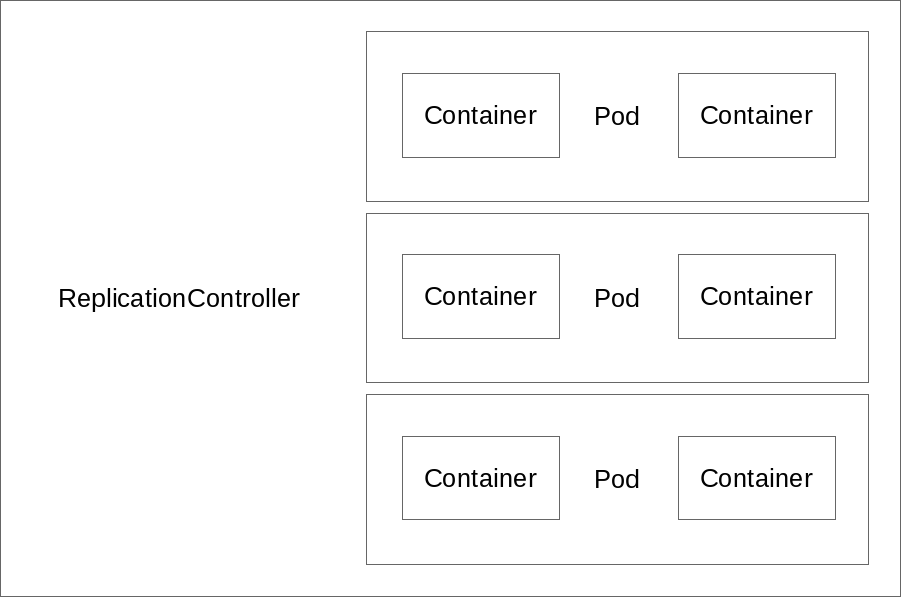
\includegraphics{media/ch5-pods-rcs.png}
\caption{Pods and Replication Controllers}
\end{figure}

A basic example of pod composed by 2 containers could be an application server and a Redis instance for caching from database.

In Gasista Felice every component is composed by a pod, a replicationController and a service for providing access to it.  Since there are 4 components, a minimal instance of the application includes 4 service, 4 replication controller and 4 pods.  The number of the pods could be changed dynamically.

Kubernetes stores the data about pods, replication controllers and services into Etcd under the \texttt{/kubernetes.io} key.

In order to add these features, Kubernetes build on top of Docker, Etcd and Flannel, adding 3 master components:

\begin{itemize}
\item \textit{API Server} validates and configures the data for pods, services, and replication controllers
\item \textit{Controller Manager} watches Etcd for changes to replication controller and then uses the API to enforce the desired state
\item \textit{Scheduler} schedule the pods into nodes depends on resources availability or other parameters
\end{itemize}

And 2 more components in nodes:

\begin{itemize}
\item \textit{Kubelet} applies changes to the node as specified in local Etcd, and updated the data on Etcd depending on local state of containers
\item \textit{Proxy} manages the services defined in Etcd on that node
\end{itemize}

\begin{figure}[htbp]
\centering
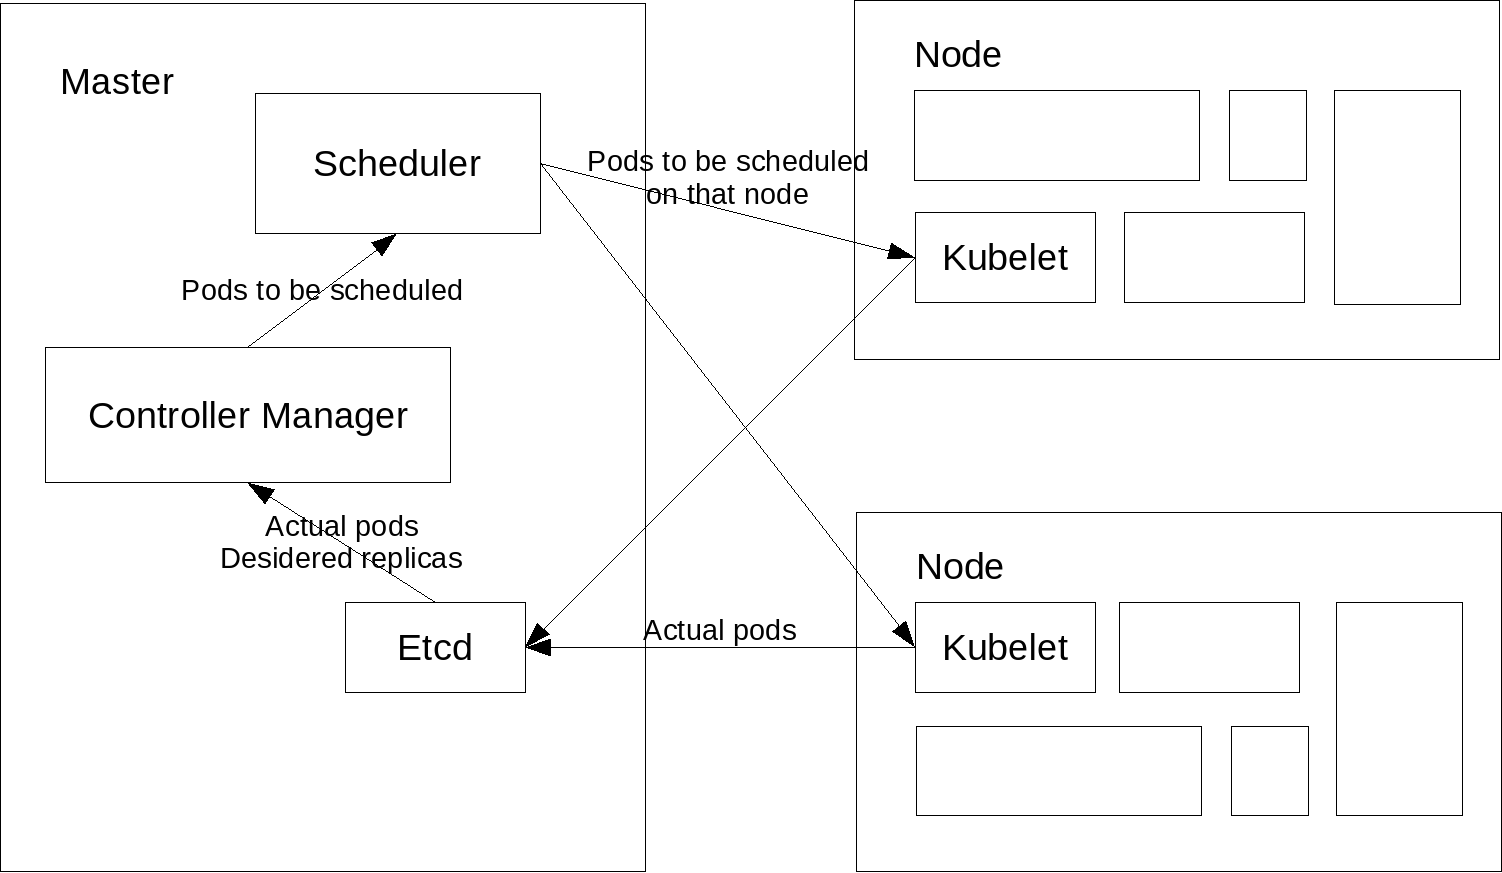
\includegraphics{media/ch5-scheduling.png}
\caption{Replicas and Scheduling}
\end{figure}

\begin{figure}[htbp]
\centering
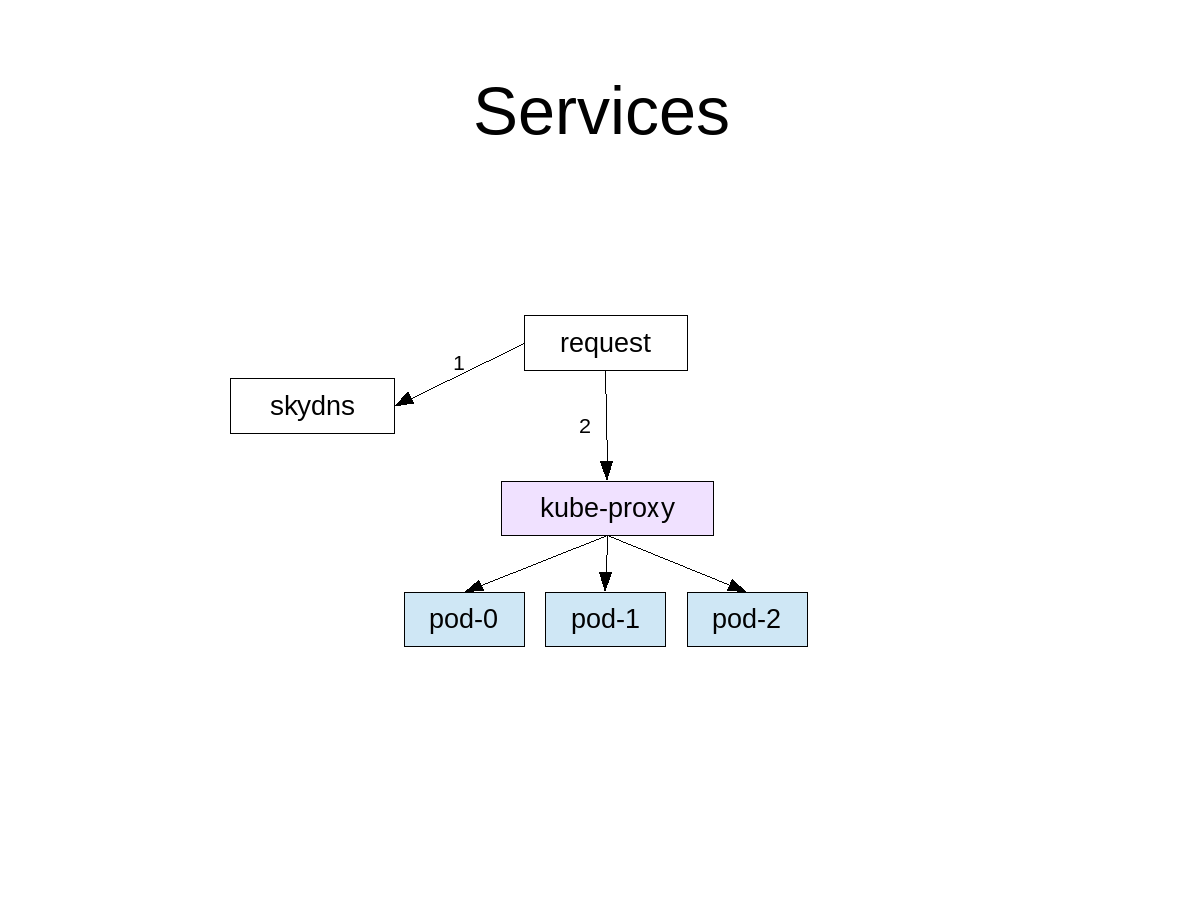
\includegraphics{media/ch5-services.png}
\caption{Scaling Pods with Kubernetes services}
\end{figure}

On July 20, 2015 the \textit{Linux Foundation} announced the \textit{Cloud Native Computing Foundation}\cite{CloudNativeComputingFoundation} in order to standardize the orchestration of components in a cloud environment, taking Kubernetes as one of the starting point.

\section{PaaS for Deploying Applications}\label{paas-for-deploying-applications}

Even if Kubernetes represents a great solution for scaling services, it lacks the concept of application and
the development workflow, so it's more a tool for system specialists. In order to reach a PaaS abstraction and deploying real applications, there is needed another level on top of Kubernetes.

The 3rd version of \textit{OpenShift} is a PaaS built on top of Kubernetes and Docker, providing a solution covers continuous delivery for modern containers and microservices world.

OpenShift extends Kubernetes APIs with additional concepts:

\begin{itemize}
\item \textit{route} configure a public DNS to point to a specific service
\item \textit{template} providing a way to define an application as a set of components (pods, replication controllers, services and routes), in a similar way as happens with Docker Compose
\end{itemize}

\begin{figure}[htbp]
\centering
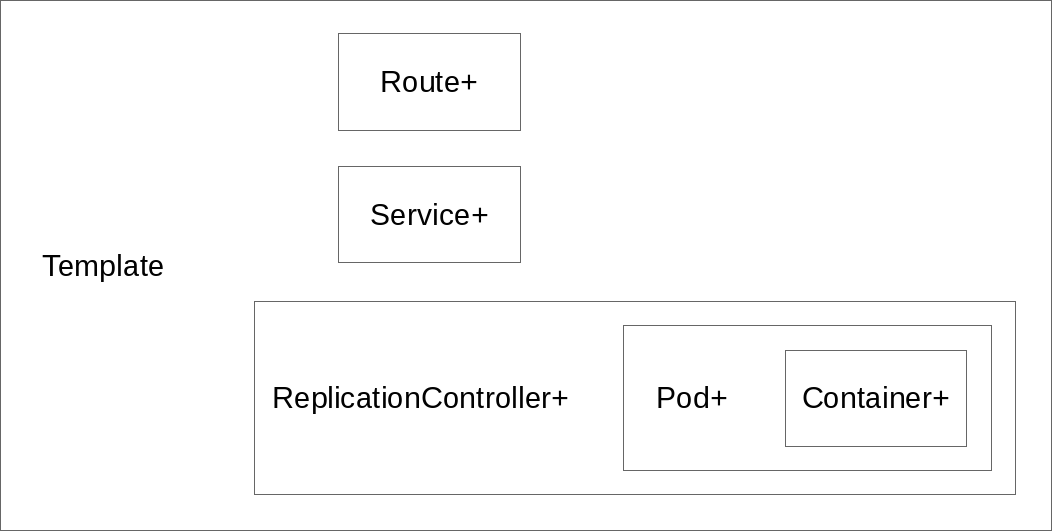
\includegraphics{media/ch5-template.png}
\caption{Route and Template objects}
\end{figure}

Gasista Felice template is composed by a total of:

\begin{itemize}
\item 4 pods (variable)
\item 4 replication controllers
\item 4 services
\item 1 route, \textit{gf.befaircloud.me} that points to proxy service
\end{itemize}

\begin{figure}[htbp]
\centering
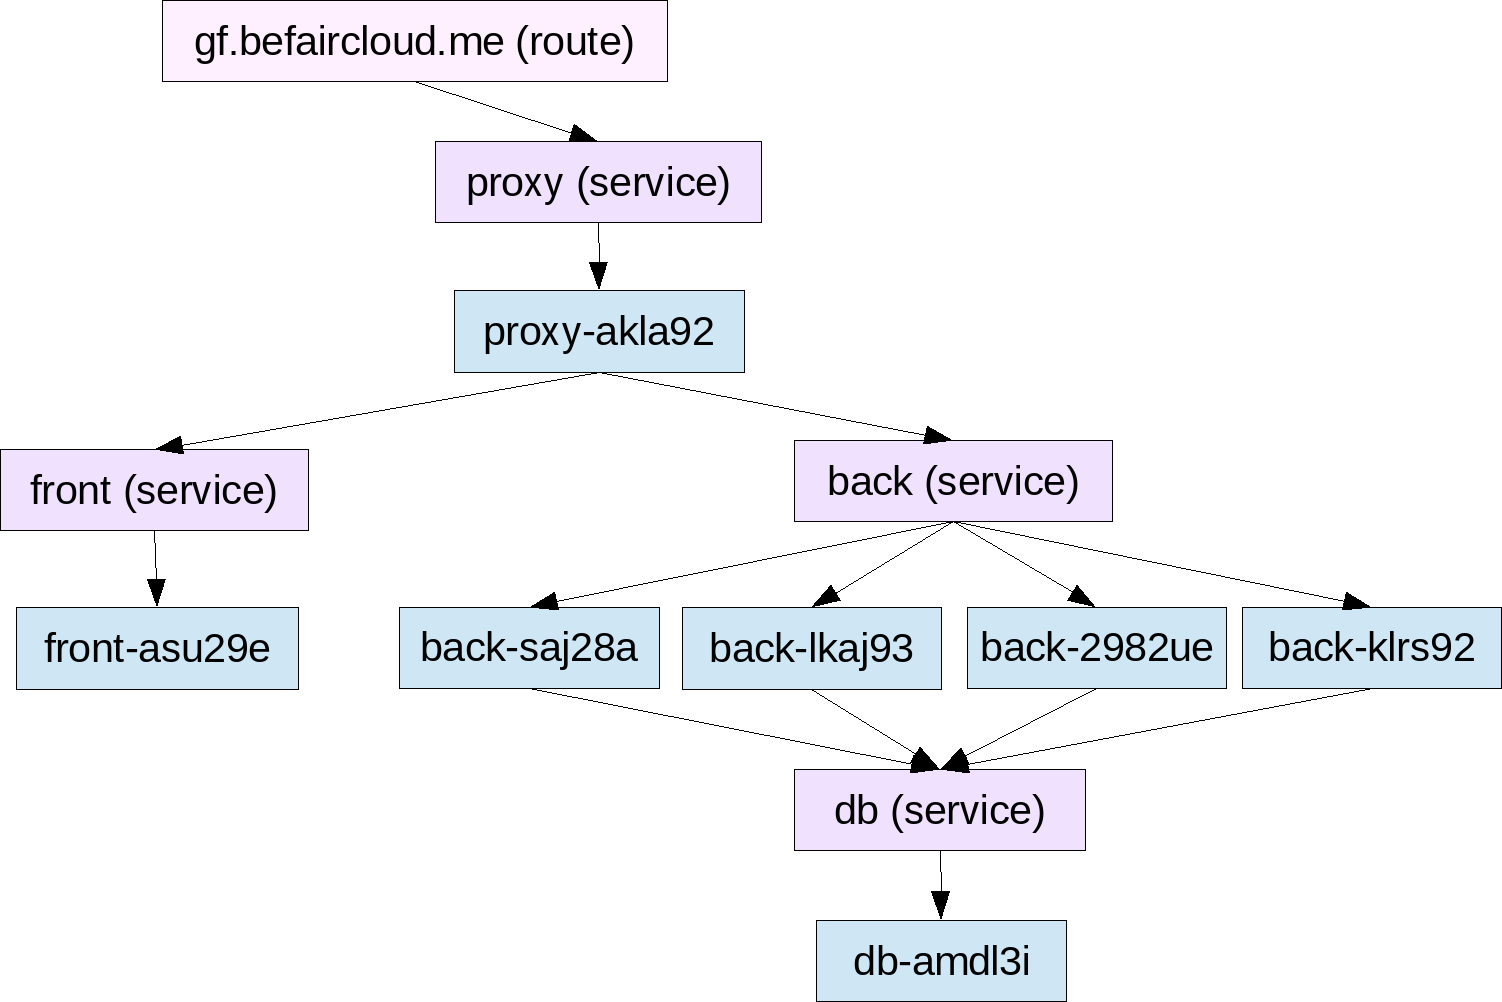
\includegraphics{media/ch5-template-gf.png}
\caption{Gasista Felice template}
\end{figure}

OpenShift stores the own objects in Etcd under \texttt{/openshift.io} key.

In order to create an instance of Gasista Felice, it needed running with \texttt{openshift/gasistafelice} script from the master.

\begin{figure}[htbp]
\centering
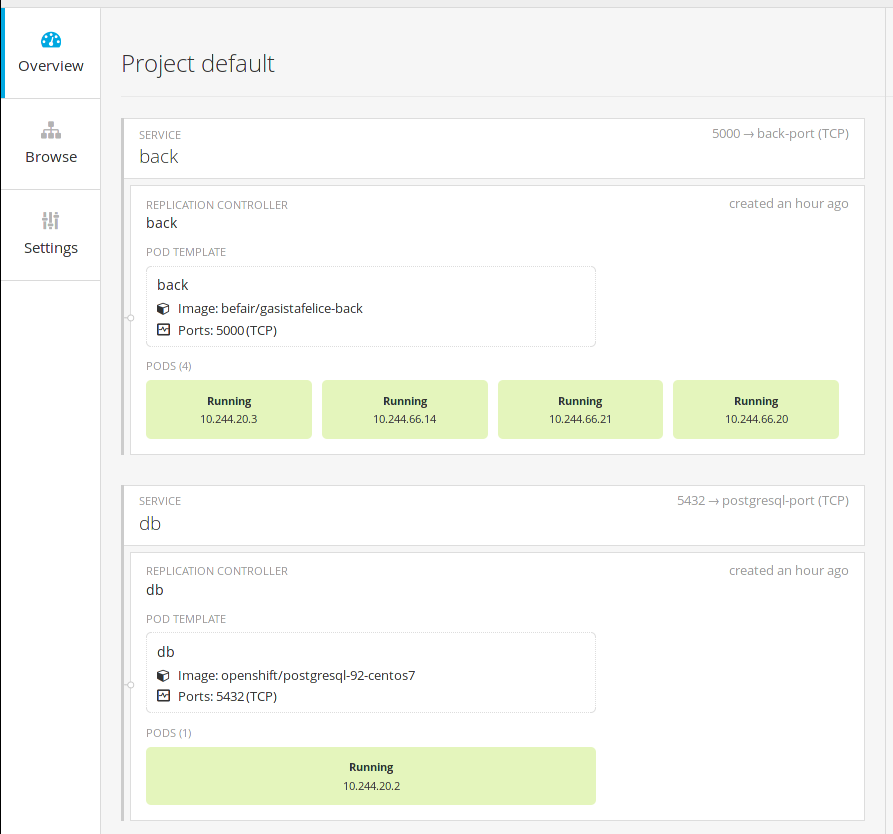
\includegraphics{media/ch5-openshift.png}
\caption{OpenShift dashboard}
\end{figure}

A small note derived on experience in deploying Gasista Felice on top of OpenShift:  while in development the default \texttt{postgresql:9.4} image worked fine, on OpenShift it had some problems probably due to permissions. So it has been used a dedicated image for OpenShift, providing PostgreSQL 9.2, also compatible with Gasista Felice.

OpenShift comes with a set of components:

\begin{itemize}
\item an \textit{HAProxy}-based external router for external reachability
\item \textit{skydns} server in order to respond to DNS queries for services
\end{itemize}

All incoming requests come to HAProxy first, than reaches the application web server, like NGINX.

Future development will include a more extensively use of OpenShift features, from built-in container image \textit{registry}, to concepts for enabling Continuous Delivery such as \textit{build}, \textit{imageStream} and \textit{deploymentConfig}.

\section{Benchmarks}\label{benchmarks}

Since Kubernetes provides the horizontal scaling of pods, that consist in adding components of the same size, will be first analyzed the Gasista Felice components from this perspective, then done some benchmarks.

The \textit{database} is the unique component that stores data.  As of other RDBMS, PostgreSQL by design is composed by a unique master, and for major scalability in reads, could be set up some slaves for future advances needs, or adding some Redis instances for caching.

The \textit{backend} there is an uWSGI application server running 4 processes of Python-based Gasista Felice backend.  This is the main pod on which it's possible act.

The \textit{frontend} is mainly useful in development, but in production once it has generated the files, it could be cached from NGINX. In further optimization, this component will be deleted at all, and the static files will be served directly. In this case will be use \texttt{1} replica since there is no need of scaling this component.

NGINX  represent the entry point of the application, so it manages caching of static content, demanding to the \texttt{front} and \texttt{back} non-cached requests. Since NGINX is generally enough fast thanks to asynchronous loops, then should not be necessary adding further pods for low to medium loads.  In a small benchmark on \texttt{http://gf.befaircloud.me/} path, with 50 concurrent request for a total of 1000 requests, the result is:  medium of 0.62s, 75.3 requests/s for a total of 13.2s.

The benchmark consist in stressing the backend, varying the number of pods.

The test consists in using \textit{boom} for 50 concurrent requests for a total of 1000 requests, that consist in a \emph{GET} at \texttt{/gasistafelice} path of the application, so a \texttt{GET\ http://gf.befaircloud.me/gasistafelice} in this case.  The test could be run with \texttt{make test} command.

Even if this should be a simple request, instead involves several work and represent a simple but significant test case. The values registered consist in:

\begin{itemize}
\item number of pods, and related uWSGI worker processes (4 uWSGI workers/pod)
\item \textit{total time}: interval from the beginning of the first request,   to the end of the last requests
\item \textit{requests per second}: represent the medium of requests served per second
\item \textit{medium}: medium of time in responding to a single request
\end{itemize}

\begin{longtable}[c]{@{}llll@{}}
\caption{Benchmark results}\tabularnewline
\toprule
Backend pods/uWSGI workers & total time & reqs/s & medium \tabularnewline
\midrule
\endfirsthead
\toprule
Backend pods/uWSGI workers & total time & reqs/s & medium \tabularnewline
\midrule
\endhead
1/4 & 647s & 1.34reqs/s & 32.0s \tabularnewline
2/8 & 410s & 2.44reqs/s & 19.8s \tabularnewline
4/16 & 297s & 3.34reqs/s & 14.3s \tabularnewline
6/24 & 202s & 4.94reqs/s & 9.71s \tabularnewline
8/32 & 185s & 5.37reqs/s & 8.85s \tabularnewline
10/40 & 175s & 5.68reqs/s & 8.35s \tabularnewline
12/48 & 186s & 5.27reqs/s & 8.69s \tabularnewline
16/64 & 194s & 5.00reqs/s & 9.09s \tabularnewline
\bottomrule
\end{longtable}

The result shows as the time decreasing from 1 to 10 pods. Beyond that number there is no advantage, probably because of cluster resource limit.